\apendice{Documentación técnica de programación}

\section{Introducción}

\section{Estructura de directorios}

\section{Manual del programador}

\section{Compilación, instalación y ejecución del proyecto}

\section{Compilación, instalación y ejecución de herramientas auxiliares}

\subsection{KEEL}

KEEL es una herramienta que permite experimentar con modelos de \textit{machine learning}. Ha sido creada por distintas universidades españolas y financiada por el Ministerio de Educación y Ciencia~\cite{KEEL}.

Para poder ejecutarla, en primer lugar, se han de descargar los ficheros fuente del repositorio de GitHub~\cite{keelRepo}. Una vez se han descargado, se compilan aprovechando el fichero \texttt{build.xmlz} contenido y la herramienta \texttt{ant}. Mediante el comando \texttt{ant cleanAll} se eliminan barios previos (para evitar conflictos), y mediante el comando \texttt{ant} se compila el código fuente.

Posteriormente se ejecuta la aplicación mediante el comando \texttt{java -jar ./dist/GraphInterKeel.jar} y se utiliza mediante su interfaz gráfica.

\begin{figure}[h]
	\caption[\textit{Co-forest}: Configuración de un experimento en KEEL]{Configuración de un experimento que utiliza el algoritmo \textit{co-forest} mediante la GUI de KEEL.}
	\centering
	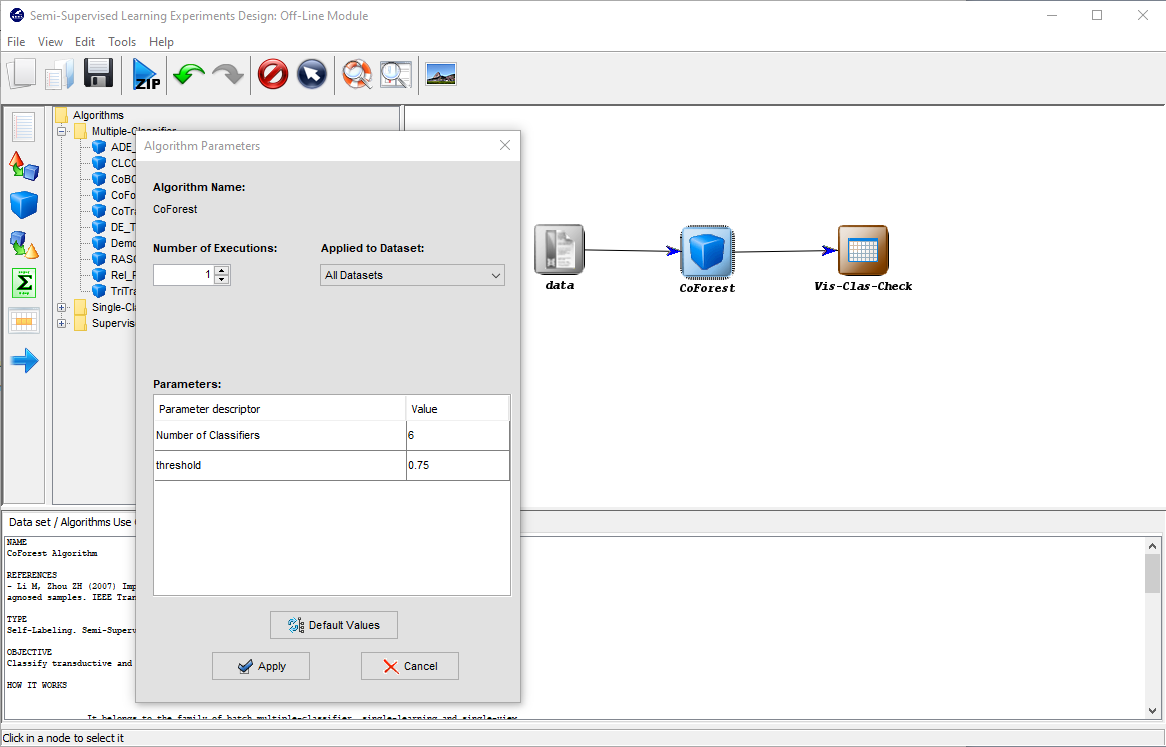
\includegraphics[width=\textwidth]{../img/anexos/manual/keel_gui.png}
\end{figure}


\section{Pruebas del sistema}

% Caso de prueba 1
\begin{table}
	\scalebox{0.80}{
		\begin{tabular}{@{}p{3em} p{6em} p{6em} p{9em} p{6em} p{6em}@{}}		
			\toprule
			\textbf{ID~CP} & 1 & \textbf{ID~RF} & 1 & \textbf{Prioridad} & Alta \\ \hline
			\multicolumn{6}{l}{\textbf{Descripción:} Esto es una descripción muy larga que se va de madre y hay un overflow segurísimo ay pues todavía no pero ahora sí} \\ \hline
			\multicolumn{6}{l}{\textbf{Precondición:}} \\ \hline
			\multicolumn{6}{l}{\textbf{Postcondición:}} \\ \hline
			\textbf{Paso} & \textbf{Acción} & \textbf{Entrada} & \textbf{Salida esperada} & \textbf{Salida real} & \textbf{Resultado}\\
			\midrule
			1 & Ir a la página de modelos & CSV mal formado & Mensaje & Mensaje & OK\\
			\bottomrule
		\end{tabular}
	}
	\caption{CP-1.0 Nombre.}
	\label{cp:nombre}
\end{table}
